\documentclass[10pt, a4paper, twoside]{basestyle}

\usepackage{tikz}
\usetikzlibrary{cd}

\usepackage[Mathematics]{semtex}
\usepackage{chngcntr}
\counterwithout{equation}{section}

%%%% Shorthands.

%%%% Title and authors.

\title{On an Article by Celledoni et al.}
\date{\printdate{2020-06-03}}
\author{Pascal~Leroy (phl)}
\begin{document}
\maketitle
\begin{sloppypar}
\noindent
This document provides clarifications, corrections, and accuracy improvements to the formulæ presented in \cite{Celledoni2007}.  It follows the notation
and conventions of that paper.  Note that the preprint \cite{Celledoni2007} differs in some of the formulæ from the final publication \cite{Celledoni2008},
but we generally follow the former.
\end{sloppypar}

\section*{Preamble}
We remind the reader of the derivation formulæ for the Jacobian elliptic functions (\cite{NistHMF2010}, section 22.13(i)):
\[
\begin{dcases}
\derivop{u}{\JacobiSN u} &= \JacobiCN u \JacobiDN u \\
\derivop{u}{\JacobiCN u} &= -\JacobiSN u \JacobiDN u \\
\derivop{u}{\JacobiDN u} &= -k^2 \JacobiSN u \JacobiCN u
\end{dcases}
\]
and for the hyperbolic functions (\cite{NistHMF2010}, section 4.34):
\[
\begin{dcases}
\derivop{u}{\HyperbolicTangent u} &= \HyperbolicSecant^2 u \\
\derivop{u}{\HyperbolicSecant u} &= -\HyperbolicSecant u \HyperbolicTangent u
\end{dcases}
\]

\section*{The equations of motion}
We start by writing equation (1) of \cite{Celledoni2007} in coordinates.  The coordinates of $\vm$ and $\VectorSymbol{I}$ are defined by:
\[
\vm\DefineAs
\begin{pmatrix}
m_1 \\ m_2 \\ m_3
\end{pmatrix}
\]
and:
\[
\VectorSymbol{I}\DefineAs
\begin{pmatrix}
I_1 & 0 & 0 \\ 0 & I_2 & 0 \\ 0 & 0 & I_3
\end{pmatrix}
\]
with $I_1 \leq I_2 \leq I_3$.

Euler's equation $\TimeDerivative{\vm} = \commutator{\vm}{\VectorSymbol{\gw}}$ can be written in coordinates in the principal axes frame:
\[
\TimeDerivative{\vm} =
\begin{pmatrix}
m_1 \\ m_2 \\ m_3
\end{pmatrix}
\times
\begin{pmatrix}
m_1/I_1 \\ m_2/I_2 \\ m_3/I_3
\end{pmatrix}
\]
thus:
\begin{equation}
\begin{dcases}
\TimeDerivative{m}_1 &= m_2 m_3 \pa{1/I_3 - 1/I_2}\\
\TimeDerivative{m}_2 &= m_3 m_1 \pa{1/I_1 - 1/I_3}\\
\TimeDerivative{m}_3 &= m_1 m_2 \pa{1/I_2 - 1/I_1}
\end{dcases}
\label{eqneuler}
\end{equation}
\section*{Solution of Euler's equation}
The solution of Euler's equation has three cases depending on the initial value of $\vm$ (more precisely, on the sign of
$\gD_2 = m_1^2 \frac{I_{12}}{I_1} + m_3^2 \frac{I_{32}}{I_3}$, see discussion below).  Figure~\ref{figm} illustrates the 
possible evolutions of $\vm$. The sphere is the surface $\norm\vm = G$, which is an invariant of motion.  The planes are
the surfaces $\gD_2 = 0$ and separate different modes of the motion.
The blue curve is called case (i) in \cite{Celledoni2007}: $\vm$ follows a periodic curve, and when that curve is close to the $m_1$
axis we have a classical case of precession.  The red curve is case (ii), and again the motion of $\vm$ is periodic and exhibits 
precession when the curve remains close to the $m_3$ axis.  The green curve is case (iii): $\vm$ takes an infinite amount
of time to reach the point $\tuple{0, G, 0}$; furthermore, the motion is unstable as any perturbation moves it either to
the blue or the red region where $\vm$ oscillates between points close to $\tuple{0, G, 0}$ and $\tuple{0, -G, 0}$; this is 
the Джанибеков effect.
\begin{figure}[htb!]
\centering
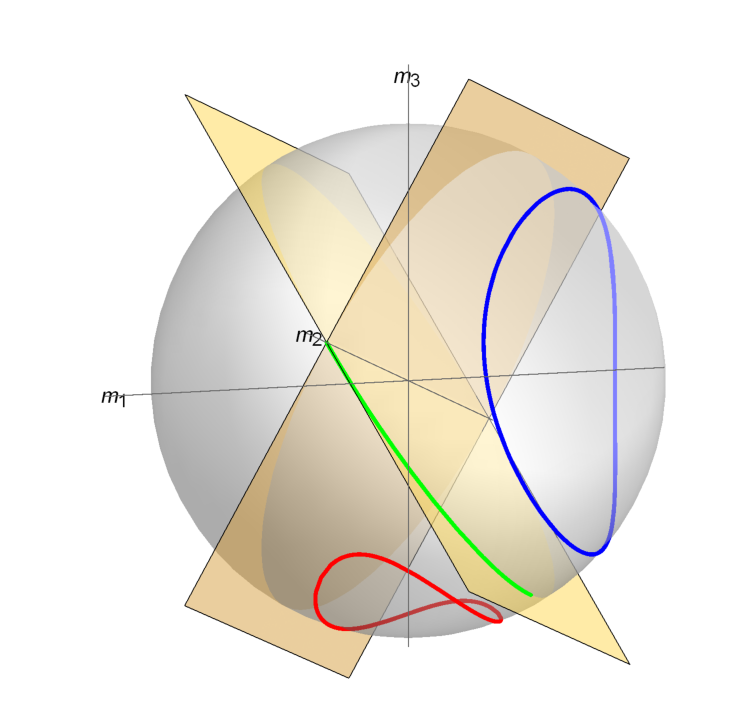
\includegraphics[scale=0.45]{Celledoni-m}
\caption{Possible trajectories of $\vm$: the blue and red curves are cases (i) and (ii), respectively, and correspond to motion
with precession.  The green curve is the (unstable) case (iii) and any perturbation demonstrates the Джанибеков effect.\label{figm}}
\end{figure}

The solutions may also be visualized by intersecting the sphere $\norm\vm = G$ with ellipsoids defined by the value of the kinetic energy $T$,
which is also a constant of motion.  Since $T = \frac{G^2 - \gD_2}{2 I_2 \Radian^2}$, different values of $T$ determine the same modes as above.
\begin{figure}[htb!]
\centering
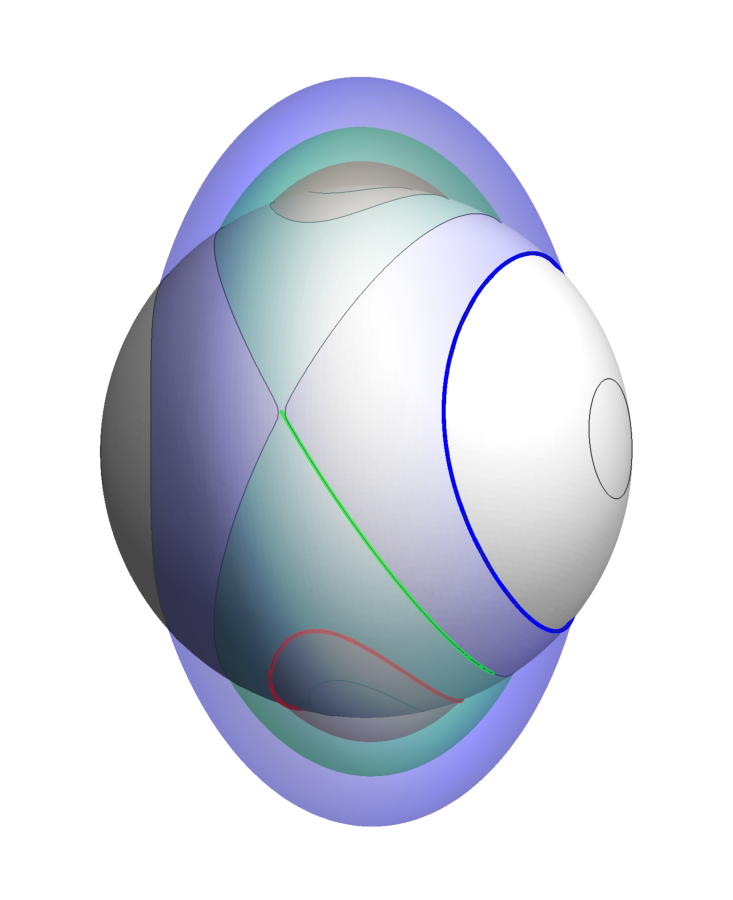
\includegraphics[scale=0.45]{Celledoni-G-T}
\caption{Possible trajectories of $\vm$: the sphere is identical to that of Figure~\ref{figm}.
The ellipsoids are surfaces of equal kinetic energy and intersect the sphere on the blue, red, and green curves depending on the
value of $T$ .\label{figGT}}
\end{figure}

In the rest of this section, we describe our notation and derive (corrected) formulæ for the three cases described above.
\subsection*{Notation}
\cite{Celledoni2007} uses a dimensionless formulation where $\norm\vm = 1$, and absolute values for $I_{jh}$ and $\gD_j$.  
We prefer to use a dimensionful formulation where $\norm\vm = G$, and to avoid absolute values.  Thus we define:
\begin{align*}
I_{jh} &\DefineAs I_j - I_h &\gD_j &\DefineAs G^2 - 2 T I_j \Radian^2 &B_{jh} &\DefineAs \sqrt{±\frac{I_j \gD_h}{I_{jh}}} \\
k &\DefineAs \sqrt{-\frac{\gD_1 I_{32}}{\gD_3 I_{21}}} &\gl_1 &\DefineAs \sqrt{\frac{\gD_1 I_{32}}{I_1 I_2 I_3}} &\gl_3 &\DefineAs \sqrt{\frac{\gD_3 I_{12}}{I_1 I_2 I_3}}
\end{align*}
With these definitions, $I_{jh} ≥ 0$ if and only if $j ≥ h$, and we will prove later that $\gD_1 ≥ 0$, $\gD_3 ≤ 0$, and that $\gD_2$ can have either sign.
The sign under the radical in the definition of $B_{jh}$ is $+$ if $h = 1$ and $j ≥ h$, or $h = 3$ and $j < h$; it is $-$ otherwise (note that we never use
$B_{j2}$ in the analysis below).  At this point it is also useful
to observe that:
\[
B_{31}^2 + B_{13}^2 = \frac{\gD_1 I_3 - \gD_3 I_1}{I_{31}} = G^2
\]

Physically, $I_{jh}$ has the dimension of a moment of inertia $\squareBrackets{L^2 M}$.  $G$ has the dimension of an angular
momentum $\squareBrackets{L^2 M T^{-1} A}$.  $T$ has the dimension of an energy $\squareBrackets{L^2 M T^{-2}}$.
$\gD_j$ has the same dimension as $G^2$.  $B_{jh}$ has the same dimension as 
$\sqrt{\gD_h}$, \idest, the same dimension as $G$.  $\gl_1$ and $\gl_3$ have the
same dimension as the quotient $\frac{G}{I_j}$, \idest, $\squareBrackets{T^{-1} A}$ which is appropriate for their usage.
\subsection*{Case (i)}
Case (i) of the solution of Euler's equation in section 2.2 of \cite{Celledoni2007} is:
\[
{\vm}_t =
\begin{pmatrix}
\gs B_{13} \JacobiDN\of{\gl t - \gn, k} \\
-B_{21} \JacobiSN\of{\gl t - \gn, k} \\
B_{31} \JacobiCN\of{\gl t - \gn, k}
\end{pmatrix}
\]
If we derive this expression with respect to $t$, inject in into (\ref{eqneuler}), and eliminate the elliptic functions we obtain:
\begin{equation}
\begin{dcases}
-\gs \gl k^2 B_{13} &= -B_{21} B_{31} \pa{1/I_3 - 1/I_2} \\
-\gl B_{21} &= \gs B_{13} B_{31} \pa{1/I_1 - 1/I_3} \\
-\gl B_{31} &= -\gs B_{13} B_{21} \pa{1/I_2 - 1/I_1}
\end{dcases}
\label{solneuleri}
\end{equation}
The last equation of (\ref{solneuleri}) yields the following value for $\gl$:
\begin{align*}
\gl &= \gs \frac{B_{13} B_{21}}{B_{31}} \frac{I_1 - I_2}{I_1 I_2}
= \gs\sqrt{\frac{I_1 \gD_3}{I_{13}} \frac{I_2 \gD_1}{I_{21}} \frac{I_{31}}{I_3 \gD_1}} \frac{I_1 - I_2}{I_1 I_2} \\
&= \gs\sqrt{\frac{-\gD_3}{I_{21} I_1 I_2 I_3}} \pa{I_1 - I_2}
= -\gs\sqrt{\frac{-\gD_3 I_{21}}{I_1 I_2 I_3}}
= -\gs \gl_3
\end{align*}
The sign change when moving $I_1 - I_2$ under the radical is necessary because $I_1 - I_2 < 0$.

It is straightforward to check that this value of $\gl$ also satisfies the other equations of (\ref{solneuleri}).  Note that it
differs in sign from the one given by \cite{Celledoni2007}: the sign error is visible in that it does not yield the proper precession 
direction.

\subsection*{Case (ii)}
Case (ii) of the solution of Euler's equation in section 2.2 of \cite{Celledoni2007} is:
\[
{\vm}_t =
\begin{pmatrix}
B_{13} \JacobiCN\of{\gl t - \gn, k^{-1}} \\
-B_{23} \JacobiSN\of{\gl t - \gn, k^{-1}} \\
\gs B_{31} \JacobiDN\of{\gl t - \gn, k^{-1}}
\end{pmatrix}
\]
Just as we did above, we derive this expression with respect to $t$, inject in into (\ref{eqneuler}), and eliminate the elliptic functions:
\begin{equation}
\begin{dcases}
-\gl B_{13} &= -\gs B_{23} B_{31} \pa{1/I_3 - 1/I_2} \\
-\gl B_{23} &= \gs B_{13} B_{31} \pa{1/I_1 - 1/I_3} \\
-\gs \gl k^{-2} B_{31} &= -B_{13} B_{23} \pa{1/I_2 - 1/I_1}
\end{dcases}
\label{solneulerii}
\end{equation}
The first equation of (\ref{solneulerii}) yields the following value for $\gl$:
\begin{align*}
\gl &= \gs \frac{B_{23} B_{31}}{B_{13}} \frac{I_2 - I_3}{I_2 I_3}
= \gs\sqrt{\frac{I_2 \gD_3}{I_{23}} \frac{I_3 \gD_1}{I_{31}} \frac{I_{13}}{I_1 \gD_3}} \frac{I_2 - I_3}{I_2 I_3} \\
&= \gs\sqrt{\frac{-\gD_1}{I_{23} I_1 I_2 I_3}} \pa{I_2 - I_3}
= -\gs\sqrt{\frac{-\gD_1 I_{23}}{I_1 I_2 I_3}}
= -\gs \gl_1
\end{align*}
Again, note the change of sign due to the fact that $I_2 - I_3 < 0$.  And again, the same value of $\gl$ can be shown to satisfy the other
equations of (\ref{solneulerii}).

\subsection*{Case (iii)}
Case (iii) of the solution of Euler's equation in section 2.2 of \cite{Celledoni2007} is clearly incorrect as it implies that $m_1$ and $m_3$
always have the same sign, whereas it is straightforward to choose initial conditions where they do not (because the separatrix is made of two
planes, see Figure~\ref{figm}).  Instead, we introduce an extra parameter $\gs'' = ±1$ and posit a solution of the form:
\[
{\vm}_t =
\begin{pmatrix}
\gs' B_{13} \HyperbolicSecant\of{\gl t - \gn} \\
G \HyperbolicTangent\of{\gl t - \gn} \\
\gs'' B_{31} \HyperbolicSecant\of{\gl t - \gn}
\end{pmatrix}
\]
Deriving this expression and injecting it into (\ref{eqneuler}) yields:
\begin{equation}
\begin{dcases}
-\gs' \gl B_{13} &= \gs'' G B_{31} \pa{1/I_3 - 1/I_2} \\
\gl G &= \gs' \gs'' B_{13} B_{31} \pa{1/I_1 - 1/I_3} \\
-\gs'' \gl B_{31} &= \gs' G B_{13} \pa{1/I_2 - 1/I_1}
\end{dcases}
\label{solneuleriii}
\end{equation}
The second equation of (\ref{solneuleriii}) gives the following value for $\gl$:
\[
\gl = \gs' \gs'' \frac{B_{13} B_{31}}{G} \frac{I_3 - I_1}{I_1 I_3}
= \gs' \gs'' \frac{1}{G} \sqrt{\frac{I_1 \gD_3}{I_{13}} \frac{I_3 \gD_1}{I_{31}}} \frac{I_3 - I_1}{I_1 I_3}
= \gs' \gs'' \frac{1}{G} \sqrt{-\frac{\gD_1 \gD_3}{I_1 I_3}}
\]
In this case it is a bit less obvious that the other equations yield the same value of $\gl$.  We detail the derivation for the first equation,
using the fact that ${\gs'}^2 = 1$:
\begin{align*}
\gl &= -\gs' \gs'' G \frac{B_{31}}{B_{13}} \frac{I_2 - I_3}{I_2 I_3}
= -\gs' \gs'' G \sqrt{\frac{I_3 \gD_1}{I_{31}} \frac{I_{13}}{I_1 \gD_3}} \frac{I_2 - I_3}{I_2 I_3} \\
&= -\gs' \gs'' G \sqrt{-\frac{\gD_1}{I_1 I_3 \gD_3}} \frac{I_2 - I_3}{I_2}
= \gs' \gs'' G \sqrt{-\frac{\gD_1}{I_1 I_3 \gD_3}} \pa{\frac{I_3}{I_2} - 1}
\end{align*}
Now note that in case (iii) we have $2 T I_2 \Radian^2 = G^2$ thus $1/I_2 = 2 T \Radian^2/G^2$.  $\gl$ can be rewritten as:
\[
\gl = \gs' \gs'' G \sqrt{-\frac{\gD_1}{I_1 I_3 \gD_3}} \pa{\frac{2 T I_3 \Radian^2}{G^2} - 1} = \gs' \gs'' \frac{1}{G} \sqrt{-\frac{\gD_1 \gD_3}{I_1 I_3}}
\]
where we have used the fact that $2 T I_3 \Radian^2 - G^2 = -\gD_3 = 2 T \Radian^2 \pa{I_3 - I_2} ≥ 0$.

We then define:
\[
\gl_2 \DefineAs \frac{1}{G} \sqrt{-\frac{\gD_1 \gD_3}{I_1 I_3}}
\]
It is easy to see that $\gl_2$ is the common value of $\gl_1$ and $\gl_3$ in case (iii), that $\gs'$ and $\gs''$ are free parameters and that:
\[
\gl = \gs' \gs'' \gl_2
\]
Note that $\gl_2$ has the same dimension as the quotient $\frac{\gD_j}{G I_j}$, which has the same dimension as $\frac{G}{I_j}$, namely, $\squareBrackets{T^{-1} A}$.

\subsection*{Phase and initial value}
The phase $\gn$ and the free parameters $\gs$, $\gs'$ and $\gs''$ are determined from the initial value ${\vm}_0$ by setting $t = 0$.
\subsubsection*{Case (i)}
We have:
\[
{\vm}_0 =
\begin{pmatrix}
\gs B_{13} \JacobiDN\of{-\gn, k} \\
-B_{21} \JacobiSN\of{-\gn, k} \\
B_{31} \JacobiCN\of{-\gn, k}
\end{pmatrix}
\]
First, we set $\gs$ to be the sign of $m_{01}$.  Then, forming the quotient of the last two coordinates we find:
\[
\frac{m_{02}}{m_{03}} = \frac{B_{21}}{B_{31}}\TrigonometricTangent\of{\JacobiAmplitude\of{\gn, k}}
\]
This equation defines $\gn$ modulo $2 K\of{k}$ because $\JacobiAmplitude\of{\gn + 2 K\of{k}, k} = \JacobiAmplitude\of{\gn, k} + \gp$  (\cite{NistHMF2010}, equation 22.16.2).  It comes:
\[
\InverseTrigonometricTangent\of{\frac{m_{02}}{m_{03}} \frac{B_{31}}{B_{21}}} = \JacobiAmplitude\of{\gn, k}
\]
and finally we obtain $\gn$ as:
\[
\gn = F\of{\InverseTrigonometricTangent\of{\frac{m_{02}}{m_{03}} \frac{B_{31}}{B_{21}}}, k}
\]
Any determination of the arc tangent works, because $F\of{\gp + \gf, k} = 2 K\of{k} + F\of{\gf, k}$ (\cite{NistHMF2010}, equation 19.2.10).  In pratice we use the \texttt{atan2} function.

\subsubsection*{Case (ii)}
Starting from:
\[
{\vm}_0 =
\begin{pmatrix}
B_{13} \JacobiCN\of{-\gn, k^{-1}} \\
-B_{23} \JacobiSN\of{-\gn, k^{-1}} \\
\gs B_{31} \JacobiDN\of{-\gn, k^{-1}}
\end{pmatrix}
\]
we set $\gs$ to be the sign of $m_{03}$ and form the quotient of the first two coordinates.  We obtain:
\[
\frac{m_{02}}{m_{01}} = \frac{B_{23}}{B_{13}} \TrigonometricTangent\of{\JacobiAmplitude\of{\gn, k^{-1}}} 
\]
and for $\gn$:
\[
\gn = F\of{\InverseTrigonometricTangent\of{\frac{m_{02}}{m_{01}} \frac{B_{13}}{B_{23}}}, k^{-1}}
\]
The same comments as above apply regarding the computation of the arc tangent.

\subsubsection*{Case (iii)}
The initial value ${\vm}_0$  is:
\[
{\vm}_0 =
\begin{pmatrix}
\gs' B_{13} \HyperbolicSecant\of{-\gn} \\
G \HyperbolicTangent\of{-\gn} \\
\gs'' B_{31} \HyperbolicSecant\of{-\gn}
\end{pmatrix}
\]
$\gs'$ and $\gs''$ are set to be the signs of $m_{01}$ and $m_{03}$, respectively.  The second coordinate immediately gives:
\[
\gn = -\InverseHyperbolicTangent\of{\frac{m_{02}}{G}}
\]

\subsection*{Implementation considerations}
Some of the formulæ given by \cite{Celledoni2007} do not lend themselves to an easy implementation or lead to numerical inaccuracies.  We
describe in this section the modifications we make to these formulæ in our implementation.

\subsubsection*{The quantity $\gD_j$}
We notice that the computation of $\gD_j$ as written in \cite{Celledoni2007} entails cancellations, so we go back to the definition of $\norm{\vm}$ and of the kinetic energy:
\[
\begin{dcases}
G^2 &= m_1^2 + m_2^2 + m_3^2 \\
2 T \Radian^2 &= \frac{m_1^2}{I_1} + \frac{m_2^2}{I_2} + \frac{m_3^2}{I_3}
\end{dcases}
\]
When, for instance, $j = 2$, this yields:
\begin{align*}
\gD_2 &= m_1^2 \pa{1 - \frac{I_2}{I_1}} + m_3^2 \pa{1 - \frac{I_2}{I_3}} \\
&= m_1^2 \frac{I_{12}}{I_1} + m_3^2 \frac{I_{32}}{I_3}
\end{align*}
and similarly:
\[
\begin{dcases}
\gD_1 &= m_2^2 \frac{I_{21}}{I_2} + m_3^2 \frac{I_{31}}{I_3} \\
\gD_3 &= m_1^2 \frac{I_{13}}{I_1} + m_2^2 \frac{I_{23}}{I_2}
\end{dcases}
\]
It is easy to see that $\gD_1$ and $\gD_3$ are the sums of terms of the same sign, so they can be computed without cancellations.  Furthermore,
$\gD_1 \geq 0$ and $\gD_3 \leq 0$.  $\gD_2$ can have either sign, which correspond exactly to cases (i) ($\gD_2 < 0$), (ii) ($\gD_2 > 0$) and 
(iii) ($\gD_2 = 0$).

\subsubsection*{The elliptic modulus}
For the computation of the elliptic functions and integrals \cite{Celledoni2007} gives the value of the elliptic modulus $k$ but we need the value of
the complementary parameter $m_c = 1 - m$ (see \cite{NistHMF2010}, section 19.1.2 for an overview of the notation).  In case (i) we have:
\[
m_c = 1 - k^2 = 1 + \frac{\gD_1 I_{32}}{\gD_3 I_{21}}
\]
This can be rewritten as follows:
\begin{align*}
m_c &= \frac{\gD_3 I_{21} + \gD_1 I_{32}}{\gD_3 I_{21}}
=\frac{\pa{G^2 - 2 T I_3}\pa{I_2 - I_1} + \pa{G^2 - 2 T I_1}\pa{I_3 - I_2}}{\gD_3 I_{21}} \\
&=\frac{G^2\pa{I_3 - I_1} + 2 T I_2\pa{I_1 - I_3}}{\gD_3 I_{21}}
=\frac{\gD_2 I_{31}}{\gD_3 I_{21}}
\end{align*}

Similarly, in case (ii):
\[
m_c = 1 - k^{-2} = 1 + \frac{\gD_3 I_{21}}{\gD_1 I_{32}}
=\frac{\gD_1 I_{32} + \gD_3 I_{21}}{\gD_1 I_{32}}
=\frac{\gD_2 I_{31}}{\gD_1 I_{32}}
\]
In both cases we have $m_c \geq 0$.

\section*{Integration of the rotation matrix}
In order to be compatible with our geometrical libraries, our notation differs from that of \cite{Celledoni2007}.
\subsection*{Notation}
\cite{Celledoni2007} describe the physical space as a three-dimensional vector space where vectors like $\VectorSymbol M$ live.  In this vector space,
they pick orthonormal bases like $\curlyBrackets{\VectorSymbol{E}^b_1, \VectorSymbol{E}^b_2, \VectorSymbol{E}^b_3}$ which they identify with the
canonical basis of $\Reals^3$ to obtain a coordinate representation $\vm$ of $\VectorSymbol M$.

They then define active rotations in the physical (vector) space.  For instance they explain that $\mathscr P_t$ takes $\VectorSymbol M$ to ${\VectorSymbol E}^b_3$ and transforms the basis $\mathscr B_t$ into the basis $\mathscr B^b$.  By contrast, our libraries operate on coordinate
representations, not abstract vectors, and implement passive rotations where the physical space is represented by multiple copies of $\Reals^3$ with
different coordinate systems.  Therefore, we view $\mathscr P_t$ as transforming $\VectorSymbol M$ with coordinates $\vm$ in the coordinate system 
$\mathscr B^b$ of the body into $\VectorSymbol M$ with coordinates $\ve_3$ in the coordinate system $\mathscr B_t$.  Confusingly, 
\cite{Celledoni2007} appear to use passive rotations when they write matrices, so their $P_t$ has semantics similar to that of our $\mathscr P_t$.

In what follows (and in our code) we try to use the same symbols as \cite{Celledoni2007} with the understanding that our rotations, written in
script font, are passive, and that the entities denoted by $\mathscr B$ are coordinate systems in multiple copies of $\Reals^3$, not bases in a 
single vector space.

\cite{Celledoni2007} decompose the attitude rotation $\mathscr Q_t$ of the body as follows:
\[
\begin{tikzcd}
{\mathscr Q_t: \mathscr B^b} \arrow{r}{\mathscr P_t} & {\mathscr B_t} \arrow{r}{\mathscr Y_t} & {\mathscr B'} \arrow{r}{\mathscr R} & {\mathscr B^s}
\end{tikzcd}
\]
where $\mathscr P_t$ maps $\vm$ onto $\ve_3^b$, $\mathscr Y_t$ is a rotation of angle $\gy\of{t}$ around $\vm$, and ${\mathscr R}$
maps $\ve_3^s$ onto $\vm$, where they assume that $\mathscr Q_{t_0} = \Identity$.  This yields the following decomposition for
$\mathscr R$:
\[
\begin{tikzcd}
{\mathscr R: \mathscr B'} \arrow{r}{\mathscr Y_{t_0}^{-1} = \Identity} & {\mathscr B_t} \arrow{r}{\mathscr P_{t_0}^{-1}} & {\mathscr B^b}
\end{tikzcd}
\]
This is not sufficient for our purpose, however, because in practical situations $\mathscr Q_{t_0}$ cannot be chosen.  Therefore we
decompose $\mathscr R$ as follows:
\[
\begin{tikzcd}
{\mathscr R: \mathscr B'} \arrow{r}{\mathscr Y_{t_0}^{-1} = \Identity} & {\mathscr B_t} \arrow{r}{\mathscr P_{t_0}^{-1}} & {\mathscr B^b}
\arrow{r}{\mathscr Q_{t_0}} & {\mathscr B^s}
\end{tikzcd}
\]

\cite{Celledoni2007} derive the following expression for $\TimeDerivative{\gy}\of{t}$ (which they write slightly differently):
\begin{align*}
\TimeDerivative{\gy}\of{t} &= \frac{2 T \Radian^2}{G} + \frac{\gD_2}{G I_2}\pa{\frac{1}{1 + \frac{I_{12}I_{23}G^2}{I_2^2 \gD_1 \gD_3}m_2^2}}\\
&= \frac{2 T \Radian^2}{G} + \frac{\gD_2}{G I_2}\pa{\frac{1}{1 - \frac{G^2}{B_{21}^2 B_{23}^2}m_2^2}}
\end{align*}

\subsection*{Case (i)}
In case (i) we have $m_2 = -B_{21} \JacobiSN\of{\gl t - \gn, k}$ and the above expression becomes:
\[
\TimeDerivative{\gy}\of{t} = \frac{2 T \Radian^2}{G} + \frac{\gD_2}{G I_2}\pa{\frac{1}{1 - \frac{G^2}{B_{23}^2}\JacobiSN^2\of{\gl t - \gn, k}}}
\]
This expression can be integrated using formula 110.04 of \cite{ByrdFriedman1954} with $\ga = G/B_{23}$ to yield:
\[
\gy\of{t} = \frac{2 T \Radian^2}{G}t + \frac{\gD_2}{\gl G I_2}\EllipticPi\of{\JacobiAmplitude\of{\gl t - \gn, k}, \frac{G^2}{B_{23}^2}, k}
\]
Note that this differs from the formula given by \cite{Celledoni2007} in the value of $n$.

\subsection*{Case (ii)}
In case (ii) we have $m_2 = -B_{23} \JacobiSN\of{\gl t - \gn, k^{-1}}$ and a computation similar to the one above gives:
\[
\TimeDerivative{\gy}\of{t} = \frac{2 T \Radian^2}{G} + \frac{\gD_2}{G I_2}\pa{\frac{1}{1 - \frac{G^2}{B_{21}^2}\JacobiSN^2\of{\gl t - \gn, k^{-1}}}}
\]
and:
\[
\gy\of{t} = \frac{2 T \Radian^2}{G}t + \frac{\gD_2}{\gl G I_2}\EllipticPi\of{\JacobiAmplitude\of{\gl t - \gn, k^{-1}}, \frac{G^2}{B_{21}^2}, k^{-1}}
\]

\subsection*{Case (iii)}
In case (iii) we have $m_2 = G \HyperbolicTangent\of{\gl t - \gn}$ and:
\[
\TimeDerivative{\gy}\of{t} = \frac{2 T \Radian^2}{G} + \frac{\gD_2}{G I_2}\pa{\frac{1}{1 - \frac{G^4}{B_{21}^2 B_{23}^2} \HyperbolicTangent^2\of{\gl t - \gn}}}
\]
which can be integrated using:
\[
\int{}\frac{1}{1 - n \HyperbolicTangent^2\of{\gl t - \gn}}\diffd{t} = 
\frac{t}{1 - n} - \frac{\sqrt{n}}{\pa{1 - n}\gl} \InverseHyperbolicTangent\of{\sqrt{n} \HyperbolicTangent\of{\gl t - \gn}}
\]

\subsection*{Implementation considerations}
The approach in this section relies on the intermediate basis $\set{\vm, \TimeDerivative{\vm}, \commutator{\vm}{\TimeDerivative{\vm}}}$.  
Unfortunately, it is not suitable for a practical implementation because it has an essential singularity when $\TimeDerivative{\vm} = \VectorSymbol{0}$:
while the condition $\TimeDerivative{\vm} = \VectorSymbol{0}$ is physically a constant of motion, $\TimeDerivative{\vm}$ itself is not.  This means that
any inaccuracies in numerical computations of $\TimeDerivative{\vm}$ (cancellations, underflow) may cause it to switch from $\VectorSymbol{0}$ to
non-$\VectorSymbol{0}$ and back.

When $\TimeDerivative{\vm} = \VectorSymbol{0}$ at $t = 0$, the motion may be computed at all times assuming a constant $\vm$, so the singularity may be
eliminated.  But when $\TimeDerivative{\vm} \neq \VectorSymbol{0}$ at $t = 0$ and it later becomes $\VectorSymbol{0}$, there is no way to find a basis at $t$ that 
continuously corresponds to the one at $t = 0$.

While it might be possible to deal with the neighbourhoods of the stable zeros ($m_1$ and $m_3$) by handling the relevant regions with distinct 
formulæ (\exempligratia, the low-order precession approximations), this is infeasible for $m_2$ where any neighbourhood of the singularity propagates all the
way around the separatrix.  The reader is invited to consult figure~\ref{figm}.

In conclusion, we tried to use this approach but had to abandon it because of the impossibility of handling the singularity.

\section*{Integration of the quaternion}
\cite{Celledoni2007} use a rotation $\mathscr P_t$ to map $\vm$ onto $\VectorSymbol{e_3}$ and obtain the following quaternionic representation for that rotation:
\[
\begin{dcases}
p_1 &= \frac{p_3 m_1 + p_0 m_2}{G + m_3} \\
p_2 &= \frac{p_3 m_2 - p_0 m_1}{G + m_3} \\
p_0^2 + p_3^2 &= \frac{G + m_3}{2 G}
\end{dcases}
\]
and the angle $\gy\of{t}$ for the rotation $\mathscr Y_t$ around $\VectorSymbol{e_3}$:
\[
\TimeDerivative{\gy}\of{t} = \frac{2 T \Radian^2 + G m_3 / I_3}{G + m_3} + 4 G \frac{p_3 \TimeDerivative{p_0} - p_0 \TimeDerivative{p_3}}{G + m_3}
\]
Solving these equations they obtain:
\[
\begin{dcases}
p_0 &= \sqrt\frac{1 + m_3/G}{2} \\
p_1 &= \frac{m_2}{\sqrt{2 G\pa{G + m_3}}} \\
p_2 &= \frac{-m_1}{\sqrt{2 G\pa{G + m_3}}} \\
p_3 &= 0
\end{dcases}
\]
and:
\[
\gy\of{t} = \frac{G}{I_3}t + \frac{G I_{31}}{\gl I_1 I_3}
\pa{\EllipticPi\of{\JacobiAmplitude\of{\gl t - \gn, k}, -\pa{\frac{B_{31}}{B_{13}}}^2, k} + f\of{t}}
\]

They note that these formulæ are only applicable if $m_3 \neq -G$ but go on applying them to case (i) where $m_3 = B_{31} \JacobiCN\of{\gl t - \gn, k}$ can be negative.

One should note at this point that \cite{Celledoni2007} make an error when copying the definition of $f_1\of{u}$ from formula 361.54 of 
\cite{ByrdFriedman1954}.  This error is corrected in \cite{Celledoni2008}, but the sign of $f\of{s}$ in the definition of $\gy\of{t}$ is
still incorrect and should read:
\[
f\of{s} \DefineAs -B_{31} \frac{B_{13}}{B_{21}} \InverseTrigonometricTangent\of{\frac{B_{21}}{B_{13}} \JacobiSD\of{\gl s - \gn, k}}
\]

\section*{An alternative quaternionic solution}
\cite{Celledoni2007} do not explain how they handle cases (ii) and (iii).  It is intriguing to note, though, that the formulæ above work well
for case (ii) where $m_3 = \gs B_{31} \JacobiDN\of{\gl t - \gn, k^{-1}}$.  The reason is that, without loss of generality, we can apply to the principal
axes of the body a rotation $\mathscr S$ that maps $m_3$ onto $-m_3$ (there are many possible choices for $\mathscr S$, but for simplicity we pick one that flips the sign of
either $m_1$ or $m_2$).  With this rotation, the multiplier $\gs$ disappears from $m_3$ and we have $m_3 \geq 0$ for all times, which ensures that
the denominator of the quaternionic coordinates $G + m_3$ can be safely computed.  The key insight here is that the coordinate where the Jacobi funtion
$\JacobiDN$ appears does not change sign, and is therefore a better choice for rotating $\vm$ to $\VectorSymbol{e_i}$.

Observing that, in case (i), $m_1 = \gs B_{13} \JacobiDN\of{\gl t - \gn, k}$, we will construct a rotation $\mathscr S$ to make $m_1$ positive and then
a rotation $\mathscr P_t$ that maps $\vm$ onto $\VectorSymbol{e_1}$.  Similarly, in case (iii) the function $\HyperbolicSecant$ appears in the
expressions of $m_1$ and $m_3$ and is always positive, so we will construct $\mathscr S$ to make both $m_1$ and $m_3$ positive and choose $\mathscr P_t$
to map $\vm$ onto $\VectorSymbol{e_1}$ or $\VectorSymbol{e_3}$.  In the rest of this section we detail the calculations used to compute $\mathscr S$,
$\mathscr P_t$ and $\gy\of{t}$.

With the introduction of $\mathscr S$, we are effectively introducing a new base $\mathscr B^p$ for the ``preferred'' principal axes of the body, and
the rotation diagrams above are modified as follows for $\mathscr Q_t$:
\[
\begin{tikzcd}
{\mathscr Q_t: \mathscr B^b} \arrow{r}{\mathscr S} & {\mathscr B^p}\arrow{r}{\mathscr P_t} & {\mathscr B_t} \arrow{r}{\mathscr Y_t} & {\mathscr B'} \arrow{r}{\mathscr R} & {\mathscr B^s}
\end{tikzcd}
\]
And for $\mathscr R$:
\[
\begin{tikzcd}
{\mathscr R: \mathscr B'} \arrow{r}{\mathscr Y_{t_0}^{-1} = \Identity} & {\mathscr B_t} \arrow{r}{\mathscr P_{t_0}^{-1}} & {\mathscr B^p} 
\arrow{r}{\mathscr S^{-1}} & {\mathscr B^b} \arrow{r}{\mathscr Q_{t_0}} & {\mathscr B^s}
\end{tikzcd}
\] 
With this choice of $\mathscr S$, the free parameters $\gs$, $\gs'$, and $\gs''$ appearing in the three cases of the resolution of Euler's equation are all $1$.

\subsection*{Integrals}
We start by computing two integrals that are useful to obtain $\gy\of{t}$.  They are valid for $0 \le a < 1$.  As far as we can tell the following integral,
which is useful for cases (i) and (ii),
is missing from \cite{ByrdFriedman1954}:
\begin{align}
\int{}\frac{1}{1 + a \JacobiDN\of{u, k}}\diffd{u} &= \nonumber\\
\frac{1}{1 - a^2}&
\begin{aligned}[t]
\;\Biggl[&\EllipticPi\of{\JacobiAmplitude\of{u, k}, \frac{a^2 k^2}{a^2 - 1}, k} - \\
&a\sqrt\frac{1 - a^2}{a^2\pa{k^2 - 1} + 1} \InverseTrigonometricTangent\of{\sqrt\frac{a^2 \pa{k^2 - 1} + 1}{1 - a^2} \JacobiSC\of{u, k}}\Biggr]
\end{aligned}
\label{integraldn}
\end{align}
Also, the following integral is useful for case (iii):
\begin{equation}
\int{}\frac{1}{1 + a \HyperbolicSecant\of{u}}\diffd{u} = u + \frac{2 a}{\sqrt{1 - a^2}} 
\InverseTrigonometricTangent\of{\frac{a - 1}{\sqrt{1 - a^2}} \HyperbolicTangent\of{\frac{u}{2}}}
\label{integralsech}
\end{equation}

\subsection*{Case (i)}
In case (i), we define $\mathscr P_t$ to map $\vm$ onto $\VectorSymbol{e_1}$.  A computation similar to that in \cite{Celledoni2007} yields that rotation
in quaternionic form:
\[
\begin{dcases}
p_2 &= \frac{p_1 m_2 + p_0 m_3}{G + m_1} \\
p_3 &= \frac{p_1 m_3 - p_0 m_2}{G + m_1} \\
p_0^2 + p_1^2 &= \frac{G + m_1}{2 G}
\end{dcases}
\]
and, for the angle $\gy\of{t}$ of the rotation $\mathscr Y_t$ around $\VectorSymbol{e_1}$:
\[
\TimeDerivative{\gy}\of{t} = \frac{2 T \Radian^2 + G m_1 / I_1}{G + m_1} + 4 G \frac{p_1 \TimeDerivative{p_0} - p_0 \TimeDerivative{p_1}}{G + m_1}
\]
We then write $p_0 = c_0 \sqrt{1 + m_1/G}$ and $p_1= c_1 \sqrt{1 + m_1/G}$ and pick $c_0 = 1/\sqrt{2}$ and $c_1 = 0$.  The quaternion simplifies to:
\[
\begin{dcases}
p_0 &= \sqrt\frac{1 + m_1/G}{2} \\
p_1 &= 0 \\
p_2 &= \frac{m_3}{\sqrt{2 G\pa{G + m_1}}} \\
p_3 &= \frac{-m_2}{\sqrt{2 G\pa{G + m_1}}}
\end{dcases}
\]
and the angle to:
\[
\TimeDerivative{\gy}\of{t} = \frac{2 T \Radian^2 + G m_1 / I_1}{G + m_1} = \frac{G^2 - \gD_1 + G m_1}{I_1\pa{G + m_1}} = \frac{G}{I_1} - \frac{\gD_1/I_1}{G + m_1} =
\frac{G}{I_1} - \frac{\gD_1}{G I_1}\frac{1}{1 + m_1/G}
\]
Using equation (\ref{integraldn}) with $a = B_{13}/G$ and simplifying the various coefficients we obtain:
\[
\gy\of{t} = \frac{G}{I_1}t + \frac{G I_{13}}{\gl I_1 I_3}
\EllipticPi\of{\JacobiAmplitude\of{\gl t - \gn, k}, \frac{I_1 I_{32}}{I_3 I_{12}}, k} -
\InverseTrigonometricTangent\of{\sqrt\frac{I_2 I_{31}}{I_3 I_{21}} \JacobiSC\of{\gl t - \gn, k}}
\]

\subsection*{Case (ii)}
In case (ii) $\mathscr P_t$ maps $\vm$ onto $\VectorSymbol{e_3}$ and we follow the computation given in \cite{Celledoni2007}.  We repeat their results
here in dimensionful form.  The quaternion is:
\[
\begin{dcases}
p_0 &= \sqrt\frac{1 + m_3/G}{2} \\
p_1 &= \frac{m_2}{\sqrt{2 G\pa{G + m_3}}} \\
p_2 &= \frac{-m_1}{\sqrt{2 G\pa{G + m_3}}} \\
p_3 &= 0
\end{dcases}
\]
and the angle:
\[
\TimeDerivative{\gy}\of{t} = \frac{G}{I_3} - \frac{\gD_3}{G I_3}\frac{1}{1 + m_3/G}
\]
Using equation (\ref{integraldn}) with $a = B_{31}/G$ and simplifying the various coefficients we obtain:
\[
\gy\of{t} = \frac{G}{I_3}t + \frac{G I_{31}}{\gl I_1 I_3}
\EllipticPi\of{\JacobiAmplitude\of{\gl t - \gn, k^{-1}}, \frac{I_3 I_{21}}{I_1 I_{23}}, k^{-1}} +
\InverseTrigonometricTangent\of{\sqrt\frac{I_2 I_{31}}{I_1 I_{32}} \JacobiSC\of{\gl t - \gn, k^{-1}}}
\]

\subsection*{Case (iii)}
In case (iii) we start by defining $\mathscr S$ so as to make both $m_1$ and $m_3$ positive.  This is always possible, perhaps by flipping $m_2$.  We then
choose $\mathscr P_t$ to map $\vm$ onto $\VectorSymbol{e_1}$ or $\VectorSymbol{e_3}$.  Which one we pick is explained below.

Assume that we map $\vm$ onto $\VectorSymbol{e_1}$.  Then using equation (\ref{integralsech}) with $a = B_{13}/G$ and simplifying the coefficients we obtain:
\[
\begin{dcases}
\gy\of{t} &= \pa{\frac{G}{I_1} - \frac{\gD_1}{G I_1}}t - \frac{2 B_{13} \gD_1}{\gl G B_{31} I_1} 
\InverseTrigonometricTangent\of{\frac{B_{13} - G}{B_{31}} \HyperbolicTangent\of{\frac{\gl t - \gn}{2}}} \\
&= \frac{G}{I_2}t - 2 \InverseTrigonometricTangent\of{\frac{B_{13} - G}{B_{31}} \HyperbolicTangent\of{\frac{\gl t - \gn}{2}}}
\end{dcases}
\]
Because $B_{13} = G$ when $B_{31} = 0$, this formula is only usable if $B_{31} \neq 0$.  For safety, we rotate onto $\VectorSymbol{e_1}$ 
if and only if $B_{13} < B_{31}$.

Conversely when we map $\vm$ onto $\VectorSymbol{e_3}$, we have $a = B_{31}/G$ and:
\[
\gy\of{t} = \frac{G}{I_2}t + 2 \InverseTrigonometricTangent\of{\frac{B_{31} - G}{B_{13}} \HyperbolicTangent\of{\frac{\gl t - \gn}{2}}}
\]
We use this formula when $B_{13} \geq B_{31}$ so we are sure that $B_{13}$ is non-$0$.
\end{document}